\section{Resultados}
\subsection{Implementación de los modelos de aprendizaje automático}

Los experimentos realizados en la presente investigación se pueden visualizar en la plataforma de \href{https://wandb.ai/scigeo/scburning}{Weights \& Biases (W\&B)}, en la cual se 
registraron los hiperparámetros, métricas y configuraciones de hardware durante el entrenamiento de modelos de aprendizaje automático.

\subsubsection{Configuración de la Red Neuronal Convolucional (CNN).}
Para el modelo, se utilizó una arquitectura de red neuronal convolucional profunda, específicamente la arquitectura U-Net. En la siguiente configuración se define la estructura fundamental 
del modelo, incluyendo el tipo de red, el encoder preentrenado utilizado, y los detalles sobre cómo se manejan las entradas y salidas del modelo (Tabla \ref{tab:config_unet}). 

\begin{longtable}{>{\raggedright\arraybackslash}p{5cm}>{\raggedright\arraybackslash}p{3cm}>{\raggedright\arraybackslash}p{7cm}}
    \caption{Configuración del modelo U-Net} \label{tab:config_unet} \\
    \hline
    \textbf{Parámetro} & \textbf{Valor} & \textbf{Detalle} \\
    \hline
    \endfirsthead
    \hline
    \textbf{Parámetro} & \textbf{Valor} & \textbf{Detalle} \\
    \hline
    \endhead
    \hline
    \endfoot
    \hline
    \endlastfoot
    Modelo & \texttt{smp.Unet} & Es una clase que representa la arquitectura de red neuronal convolucional profunda U-Net. \\
    Nombre del encoder (\texttt{encoder\_name}) & Resnet50 & Es un modelo de red neuronal convolucional pre-entrenado. \\
    Pesos del encoder (\texttt{encoder\_weights}) & ImageNet & Es una base de datos de imágenes etiquetadas. \\
    Número de canales de entrada (\texttt{in\_channels}) & 16 & 12 bandas de Sentinel-2, BADI, NBR, Slope y Distance to Agriculture Cover \\
    Número de canales de salida (\texttt{classes}) & 1 & Imagen con las probabilidades de quema. \\
    Tasa de aprendizaje (\texttt{lr}) & 0.0001 & Tasa de aprendizaje. \\
    Peso de las clases (\texttt{class\_weights}) & [1, 15] & Peso de las clases para la función de pérdida [``no quema'', ``quema'']. \\
    Función de pérdida (\texttt{loss}) & WCE - Dice Loss & Suma ponderada entre la pérdida ponderada de entropía cruzada binaria y pérdida de DICE. \\
    Métricas de evaluación & F1, Precisión, Recall, IoU, Kappa & Métricas de evaluación en el entrenamiento y validación del modelo \\
    \hline
\end{longtable}
\begin{flushleft}
    \vspace{-\baselineskip}
    \textit{Nota.} El experimento se visualiza en \href{https://wandb.ai/scigeo/scburning/runs/62zixqn0}{Weights \& Biases}.       
\end{flushleft}

También se muestra la configuración del entrenamiento que define cómo se entrenará el modelo, especificando detalles sobre los datos 
utilizados, la estrategia de entrenamiento y los recursos computacionales. (Tabla \ref{tab:config_train_unet}):

\begin{longtable}{>{\raggedright\arraybackslash}p{5cm}>{\raggedright\arraybackslash}p{3cm}>{\raggedright\arraybackslash}p{7cm}}
    \caption{Configuración del entrenamiento del modelo UNet}  \label{tab:config_train_unet} \\
    \hline
    \textbf{Parámetro} & \textbf{Valor} & \textbf{Detalle} \\
    \hline
    \endfirsthead
    \hline
    \textbf{Parámetro} & \textbf{Valor} & \textbf{Detalle} \\
    \hline
    \endhead
    \hline
    \endfoot
    \hline
    \endlastfoot
    Dataset de entrenamiento & 675 & Conjunto de datos dividido para el entrenamiento. \\
    Dataset de validación & 168 & Conjunto de datos dividido para la validación dentro del entrenamiento. \\    
    Tamaño de lote (\texttt{batch\_size}) & 16 & Número de ejemplos de entrenamiento utilizados en una iteración. \\
    Número de workers (\texttt{num\_workers}) & 16 & Número de subprocesos (o procesos) que se crean para realizar tareas en paralelo. \\
    Estrategia de entrenamiento & ddp & Distribuye los datos a través de múltiples GPU y nodos de manera paralela en sistemas distribuidos. \\
    Tipo de aceleración & GPU & Unidades de procesamiento gráfico para realizar cálculos intensivos en paralelo. \\
    Dispositivo & 0 & GPU NVIDIA GeForce RTX 4070 con 12 GB de memoria. \\
    Número de épocas (\texttt{max\_epochs}) & 50 & Número máximo de veces que el modelo ve todo el conjunto de datos en el entrenamiento. \\
    Callbacks & ModelCheckpoint, EarlyStopping & ModelCheckpoint guarda el mejor modelo durante el entrenamiento, mientras que EarlyStopping detiene el 
    entrenamiento si no hay mejoras, para prevenir el sobreajuste. \\
    Precisión (\texttt{precision}) & 16-mixed & Precisión mixta de 16 bits en cálculos de punto flotante. \\        
    \hline
\end{longtable}
\begin{flushleft}
    \vspace{-\baselineskip}
    \textit{Nota.} El experimento se visualiza en \href{https://wandb.ai/scigeo/scburning/runs/3nfebv59}{Weights \& Biases}.     
\end{flushleft}

\subsubsection{Resultados del modelo U-Net en la detección de áreas quemadas.}
El resultado del entrenamiento de la red neuronal convolucional dio un valor de pérdida (WCE - Dice) de 0.289 para el
conjunto de datos de prueba. Cuantitativamente, el modelo UNet obtuvo valores de F1 de 67.2\%, precisión de 60.2\%, 
recall de 77.2\%, IoU de 51.1\% y Kappa de 75.7\% para el conjunto de datos de prueba.

Los resultados cualitativos se pueden visualizar la Figura \ref{fig:unet_resultados}, donde cada columna representa un caso distinto, mostrando las 
predicciones del modelo U-Net en diversos contextos de áreas quemadas.

El modelo U-Net muestra un excelente desempeño al delimitar áreas quemadas extensas en todos los casos, ya que tiende a agrupar 
los píxeles dispersos y proporcionar una delimitación más coherente, especialmente en áreas de quema menores a 10 hectáreas (\textbf{quinto caso}).

En situaciones de quemas activas (\textbf{tercer caso}) y en áreas con quema no reciente (\textbf{quinto caso}), el modelo logra 
una buena delimitación sin confundir las áreas de suelo desnudo que rodean la área con quema.

Sin embargo, en casos donde se requiere una mayor precisión para diferenciar límites de los campos de cultivo, como en el \textbf{cuarto caso}, 
el modelo tiende a subestimar la extensión de las áreas quemadas, lo que resulta en delimitaciones incorrectas.

\begin{figure}[H]
    \centering
    \caption{Resultados del modelo U-Net.}
    \label{fig:unet_resultados}
    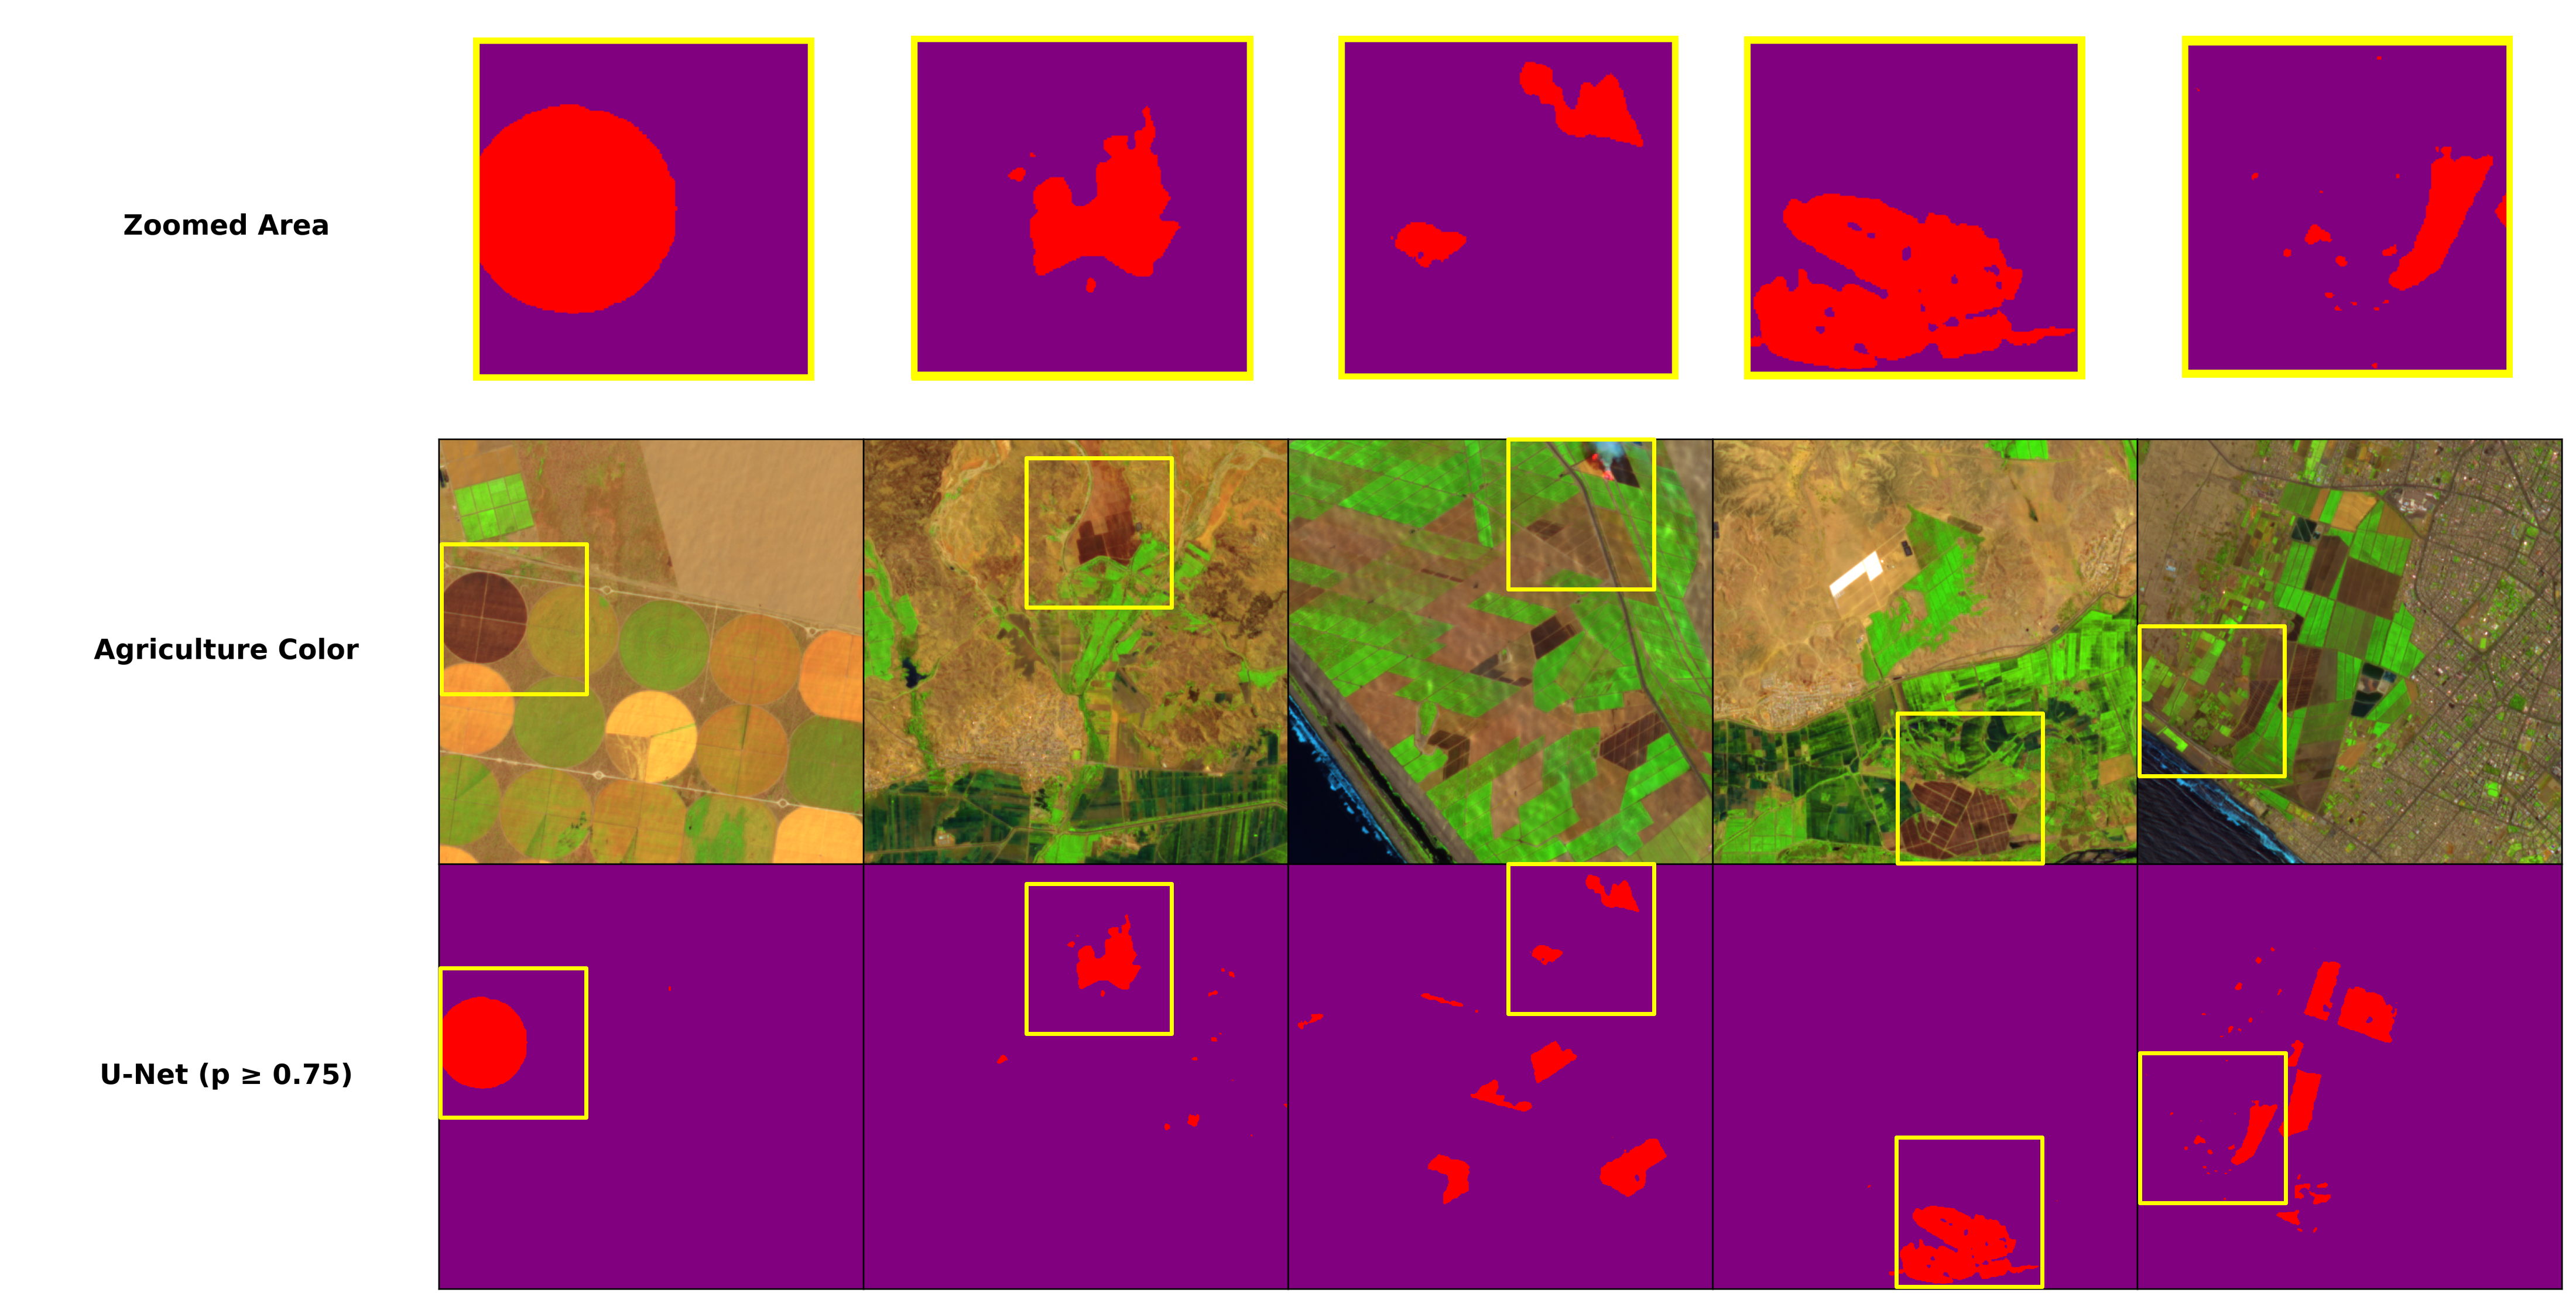
\includegraphics[width=1\textwidth]{img/7_resultados/unet_predictions.png}
    \begin{flushleft}
        \vspace{-\baselineskip}
        \textit{Nota.} El color rojo representa las áreas quemadas y el morado las áreas no quemadas. Cada caso corresponde a una columna.
        \vspace{-\baselineskip}
    \end{flushleft}
\end{figure}

\subsubsection{Configuración y resultados del Gradient Boosting Decision Tree (LightGBM).}
Para la configuración del Gradient Boosting Decision Tree dentro del framework LightGBM se consideraron las principales parámetros 
(Tabla \ref{tab:config_train_gbdt}).

\begin{longtable}{>{\raggedright\arraybackslash}p{5cm}>{\raggedright\arraybackslash}p{3cm}>{\raggedright\arraybackslash}p{7cm}}
    \caption{Principales parámetros para el entrenamiento del modelo GBDT} 
    \label{tab:config_train_gbdt} \\
    \hline
    \textbf{Parámetro} & \textbf{Valor} & \textbf{Detalle} \\
    \hline
    \endfirsthead
    \hline
    \textbf{Parámetro} & \textbf{Valor} & \textbf{Detalle} \\
    \hline
    \endhead
    \hline
    \endfoot
    \hline
    \endlastfoot
    Tarea (\texttt{task}) & train & Tarea de entrenamiento del modelo. \\
    Tipo de potenciación (\texttt{boosting\_type}) & gbdt & Árboles de decisión potenciados por gradiente. \\       
    Objetivo de destino (\texttt{objective}) & binary & Los resultados son dos clases: ``no quema'' y ``quema''. \\
    Métricas de entrenamiento (\texttt{metric}) & binary\_logloss & Pérdida logarítmica binaria también conocida como entropía cruzada binaria. \\
    Frecuencia de métricas (\texttt{metric\_freq}) & 1 & Frecuencia de métricas por cada árbol construido. \\
    Número de hojas (\texttt{num\_leaves}) & 31 & Número de hojas máximo en un árbol. \\
    Estrategia de muestreo (\texttt{data\_sample\_strategy}) & goss & Muestreo de datos utilizando el algoritmo GOSS. \\
    Tasa de aprendizaje (\texttt{learning\_rate}) & 0.5 & Tasa de aprendizaje. \\
    Fracción de características (\texttt{feature\_fraction}) & 0.9 & Fracción de características seleccionadas para la construcción de árboles. \\
    Tasa de retención de altos gradientes (\texttt{top\_rate}) & 0.2 & Se utilizarán el 20\% de los datos con los gradientes más altos para la construcción de árboles. \\
    Tasa de retención de pequeños gradientes (\texttt{other\_rate}) & 0.1 & Se utilizarán el 10\% de los datos con los gradientes más bajos para la construcción de árboles. \\
    Dispositivo (\texttt{device}) & gpu & Unidades de procesamiento gráfico para
    realizar cálculos intensivos en paralelo.\\
    ID de la plataforma (\texttt{gpu\_platform\_id}) & 0 & GPU NVIDIA GeForce RTX 4070 con
    12 GB de memoria.\\
\end{longtable}
\begin{flushleft}
    \vspace{-\baselineskip}
    \textit{Nota.} El experimento se visualiza en \href{https://wandb.ai/scigeo/scburning/runs/62zixqn0}{Weights \& Biases}.        
\end{flushleft}

Los resultados del modelo LightGBM arrojaron una pérdida logarítmica binaria de 0.155 para el conjunto de datos de prueba. 
Cuantitativamente, los resultados de las métricas de evaluación fueron F1 de 86.0\%, precisión de 79.3\%, recall de 93.8\%,
IoU de 75.4\% y Kappa de 81.2\%.

Asimismo, en la Figura \ref{fig:feature_importance}, se ilustra la importancia de las características empleadas en el modelo LightGBM. Se observa que la distancia a la cobertura agrícola (DIST\_CROPS\_COVER) 
con un 76\% y los índices de quema (BADI y NBR) con un 50\% y 46\% respectivamente son las más relevantes para la clasificación de áreas quemadas.

\begin{figure}[H]
    \centering
    \caption{Importancia de las características en el modelo LightGBM.}
    \label{fig:feature_importance}
    \includegraphics[width=1\textwidth]{img/7_resultados/feature_importance.png}
    \begin{flushleft}
        \textit{Nota.} Elaboración propia con datos de Weights \& Biases.
        \vspace{-\baselineskip}
    \end{flushleft}
\end{figure}

Para resultados cualitativos se puede visualizar la Figura \ref{fig:lightgbm_resultados}, donde cada columna representa un caso distinto, mostrando las predicciones del modelo LightGBM en diversos contextos de 
áreas quemadas.

El modelo LightGBM muestra mejoras significativas en la delimitación de áreas quemadas para grandes extensiones, especialmente en el \textbf{primer caso} y el \textbf{cuarto caso}, donde logra capturar los 
contornos de manera más precisa en comparación con el modelo U-Net.

Sin embargo, en el \textbf{segundo caso} y en el \textbf{tercer caso}, se observa una dispersión considerable de los píxeles, lo que dificulta una delimitación clara de las áreas quemadas, especialmente dentro
de las áreas quemada con características complejas, como zonas mixtas de vegetación y suelo.

En el \textbf{quinto caso}, esta dispersión se vuelve aún más pronunciada, resultando en un efecto de ruido o ``salt n' peper'' que afecta significativamente la delimitación en áreas donde las características 
espectrales del terreno circundante, como áreas de quema no reciente y suelo desnudo, son similares a las áreas quemadas.

\begin{figure}[H]
    \centering
    \caption{Resultados del modelo LightGBM.}
    \label{fig:lightgbm_resultados}
    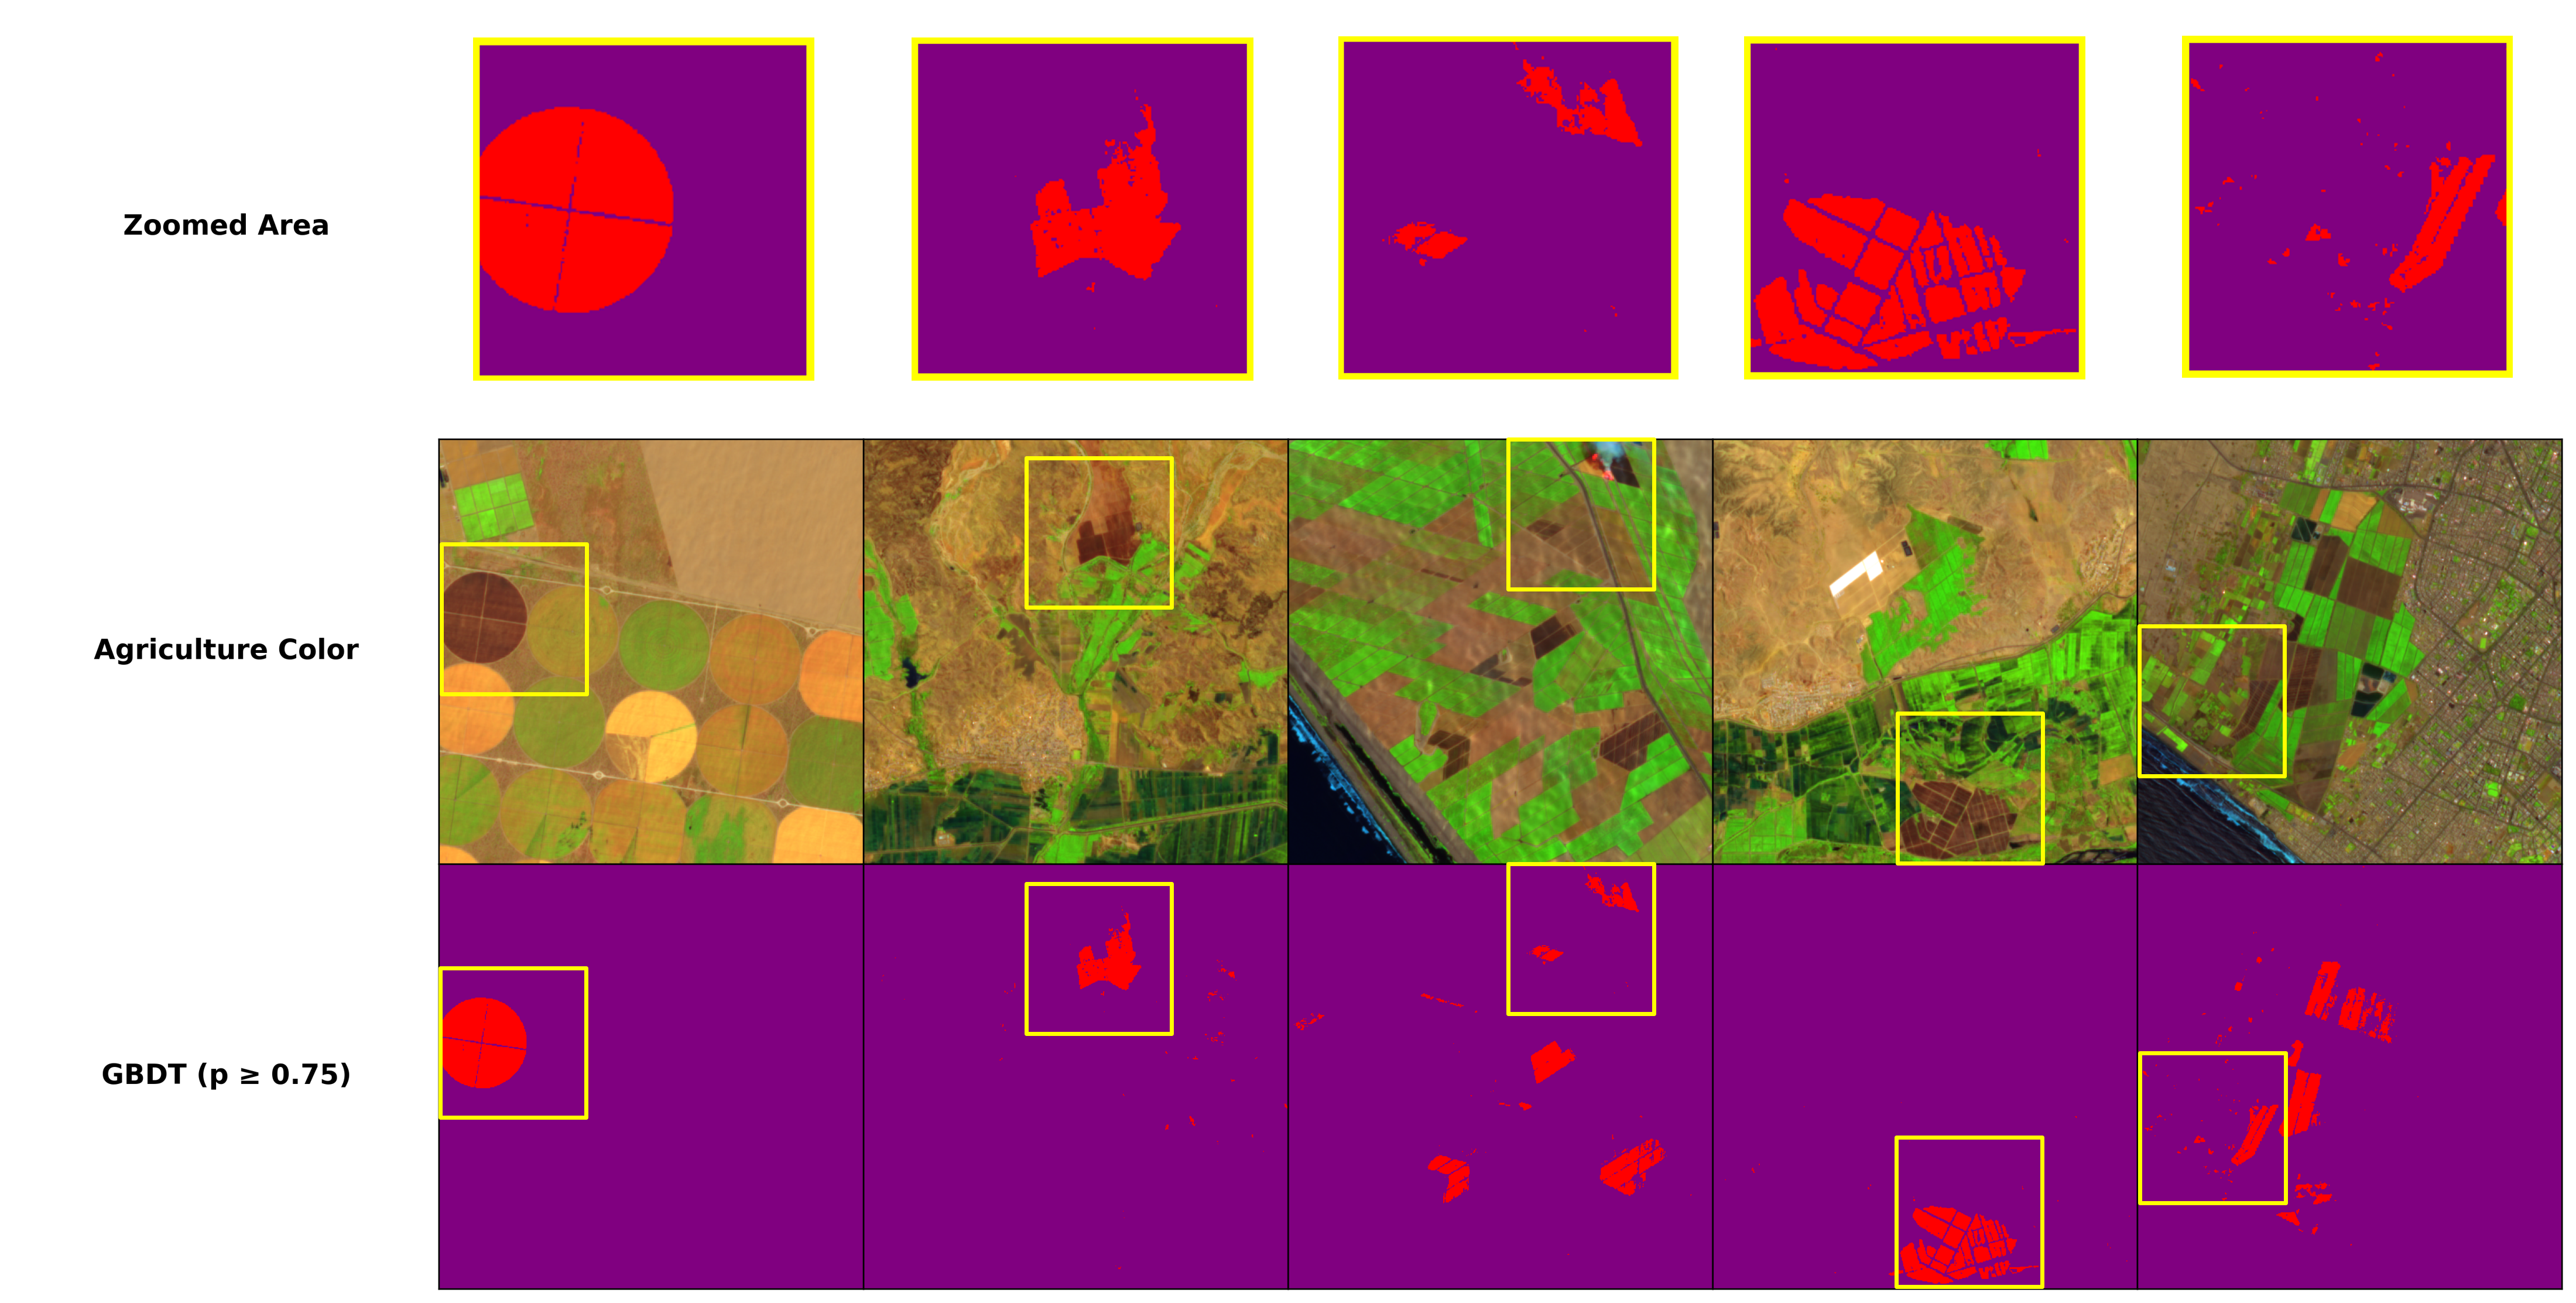
\includegraphics[width=1\textwidth]{img/7_resultados/gbdt_predictions.png}
    \begin{flushleft}
        \vspace{-\baselineskip}
        \textit{Nota.} El color rojo representa las áreas quemadas y el morado las áreas no quemadas. Cada caso corresponde a una columna.
        \vspace{-\baselineskip}
    \end{flushleft}
\end{figure}

\subsubsection{Configuración y resultados del modelo Stacking.}

Para el modelo Stacking, se utilizó como entrada los mapa de probabilidades del modelo UNet y LightGBM, y se entrenó un metamodelo de regresión 
logística con la siguiente configuración (Tabla \ref{tab:config_logistic}):

\begin{longtable}{>{\raggedright\arraybackslash}p{5cm}>{\raggedright\arraybackslash}p{3cm}>{\raggedright\arraybackslash}p{7cm}}
    \caption{Configuración del modelo de regresión logística} \label{tab:config_logistic} \\
    \hline
    \textbf{Parámetro} & \textbf{Valor} & \textbf{Detalle} \\
    \hline
    \endfirsthead
    \hline
    \textbf{Parámetro} & \textbf{Valor} & \textbf{Detalle} \\
    \hline
    \endhead
    \hline
    \endfoot
    \hline
    \endlastfoot
    Parámetro de regularización (\texttt{C}) & 1.0 & Inversa de la fuerza de regularización. \\
    Penalidad (\texttt{penalty}) & l2 & Regularización L2 para evitar el sobreajuste. \\
    Soucionador (\texttt{solver}) & lbfgs & Algoritmo de optimización para minimizar la función de pérdida (binary cross-entropy). \\    
    \hline
\end{longtable}
\begin{flushleft}
    \vspace{-\baselineskip}
    \textit{Nota.} Elaboración propia.
\end{flushleft}

Los resultados del modelo ensamblado de Stacking arrojaron una pérdida logarítmica binaria de 0.157 para el conjunto de datos de prueba. Los resultados cuantitativos de las 
métricas de evaluación fueron F1 de 90.6\%, precisión de 86.4\%, recall de 95.3\%, IoU de 82.8\% y Kappa de 87.5\%.

En la Figura \ref{fig:ensemble_resultados}, se presentan los resultados cualitativos donde cada columna representa un caso distinto, mostrando las predicciones del modelo 
Stacking en diversos contextos de áreas quemadas.

El modelo de stacking muestra resultados similares al U-Net en los tres primeros casos, logrando una buena delimitación de las áreas quemadas extensas y agrupando los 
píxeles dispersos de manera efectiva.

En el \textbf{cuarto caso}, el modelo de stacking se desempeña un poco mejor que U-Net, proporcionando una delimitación más precisa de las áreas quemadas. Sin embargo, 
no es tan claro ni detallado como el modelo LightGBM en esta situación.

En el \textbf{quinto caso}, aunque el modelo de stacking hereda los problemas del ``salt n' pepper'', logra agrupar la mayoría de este ruido, proporcionando una forma más 
clara y reduciendo en cierta medida la dispersión, lo que resulta en una delimitación más definida en las pequeñas áreas, en comparación a los otros modelos.

\begin{figure}[H]
    \centering
    \caption{Resultados del modelo ensamblado.}
    \label{fig:ensemble_resultados}
    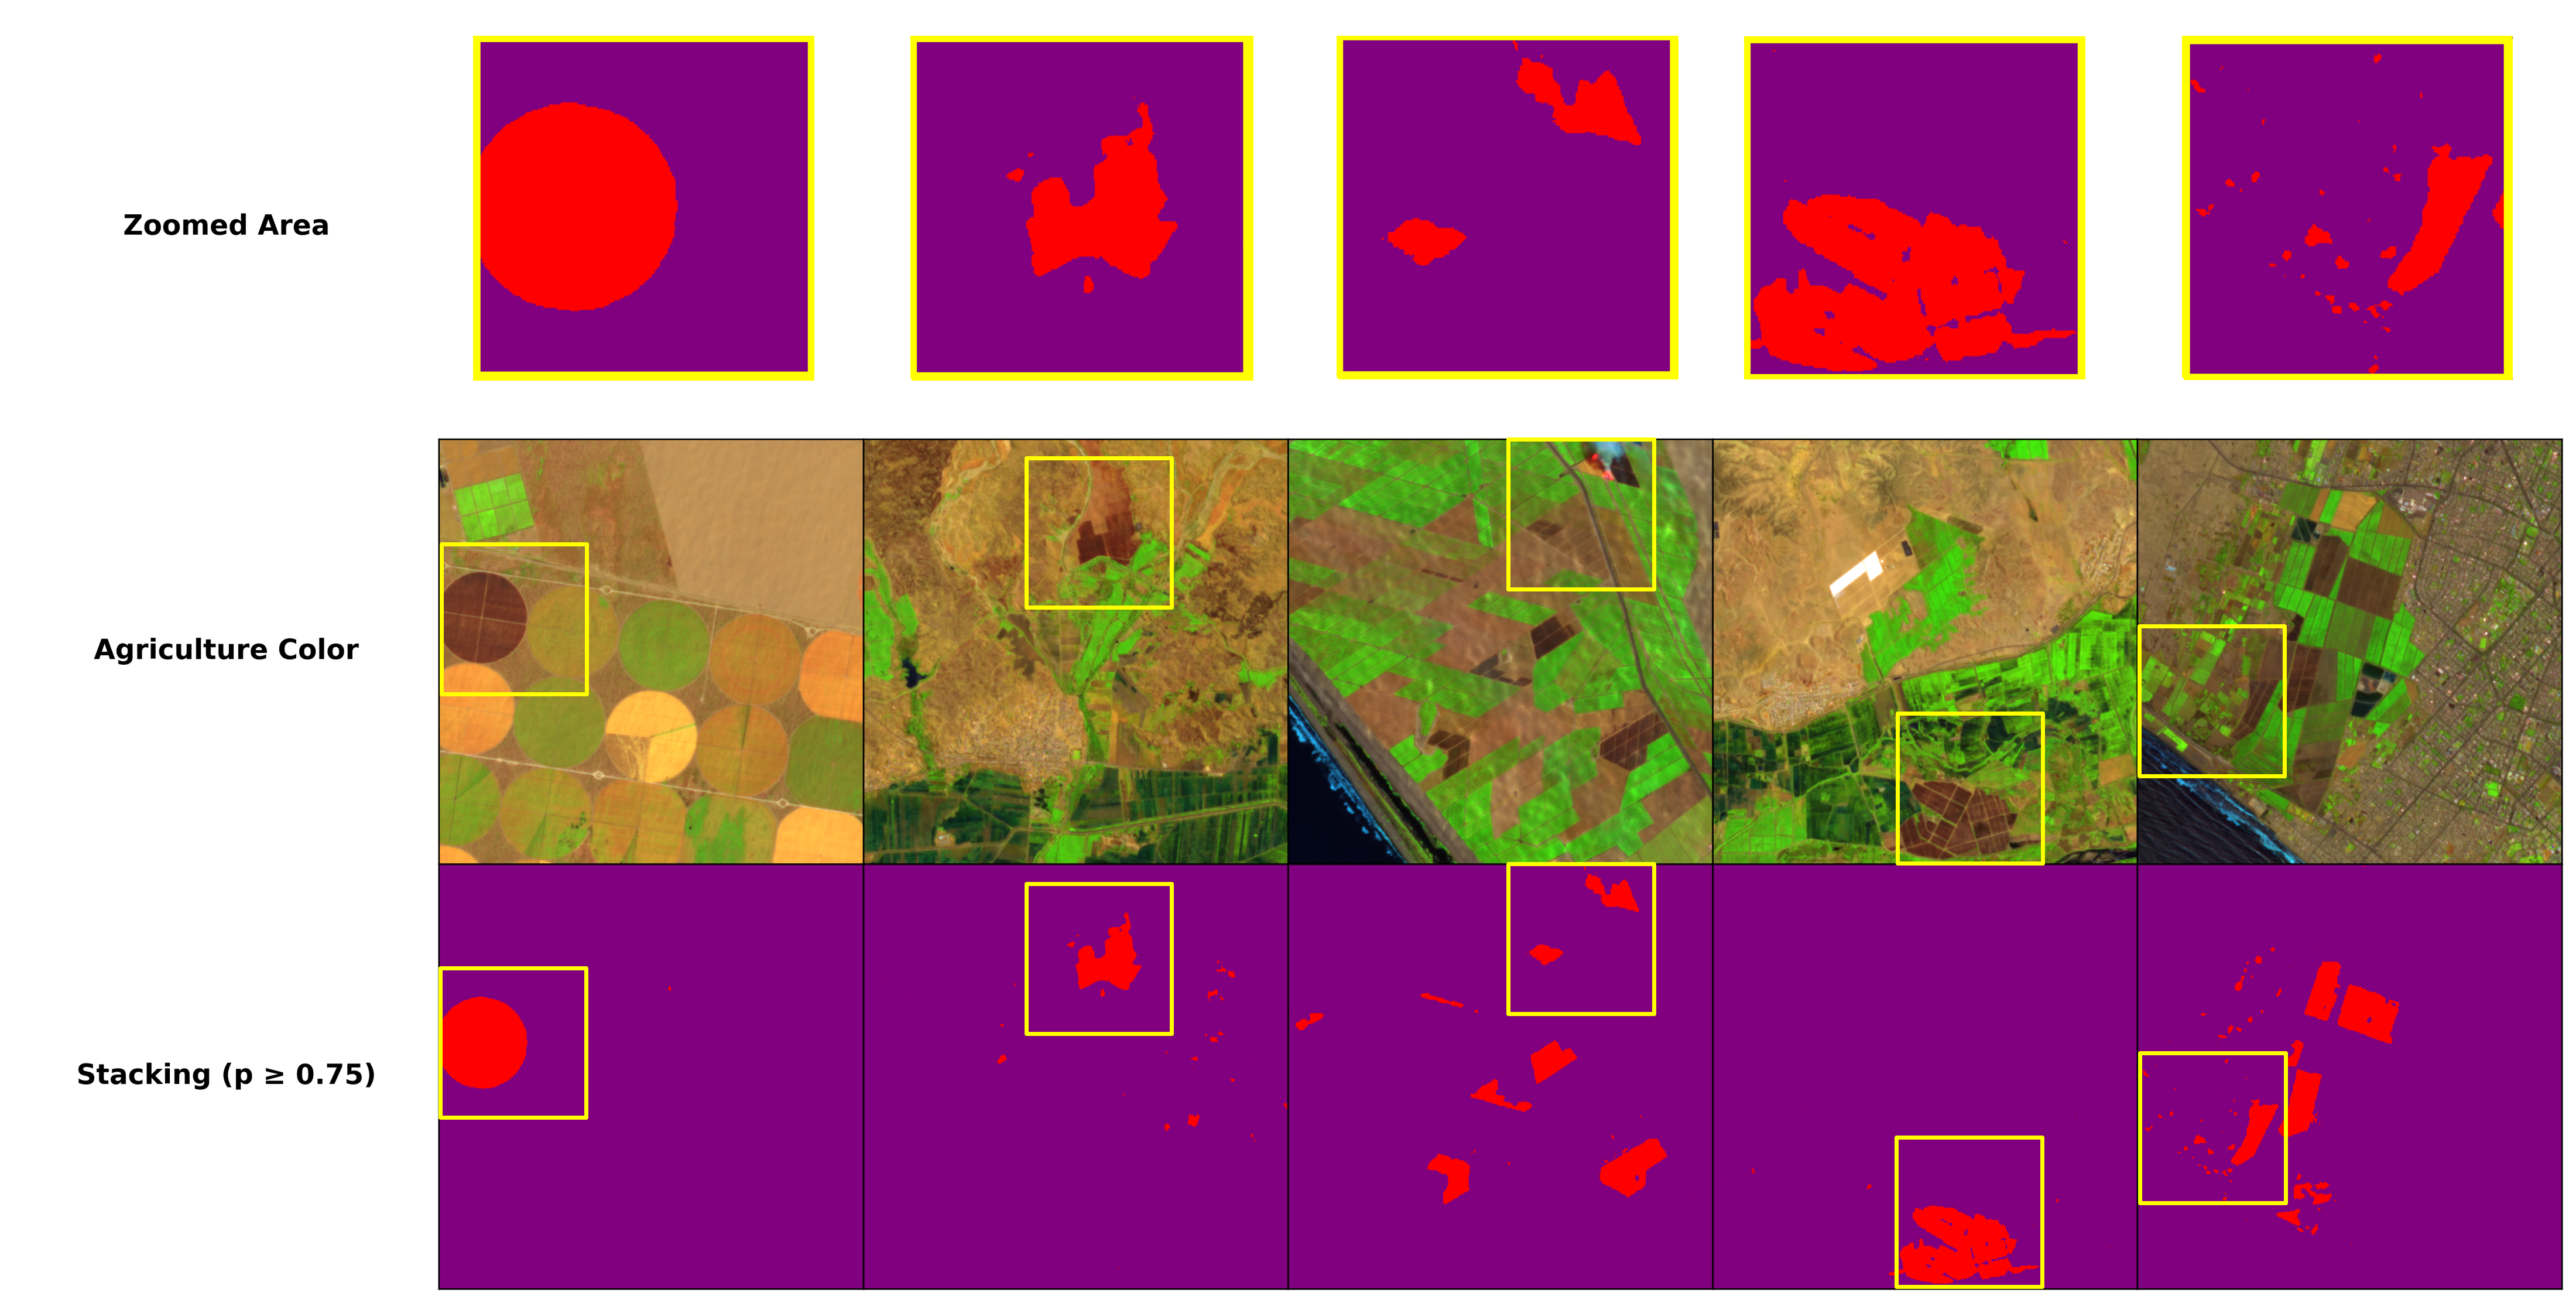
\includegraphics[width=1\textwidth]{img/7_resultados/ensemble_predictions.png}
    \begin{flushleft}
        \vspace{-\baselineskip}
        \textit{Nota.} El color rojo representa las áreas quemadas y el morado las áreas no quemadas. Cada caso corresponde a una columna.
        \vspace{-\baselineskip}
    \end{flushleft}
\end{figure}

\subsection{Evaluación de los modelos}
Para la evaluación de los modelos, se utilizó la métrica de evaluación de F1, precisión, recall, IoU y Kappa sobre el conjunto de datos de
prueba, las cuales se presentan en la Tabla \ref{tab:evaluacion_modelos}. Se observa que el modelo de Stacking supera consistentemente a U-Net y LightGBM en cada una de 
estas métricas.

\begin{table}[H]
    \centering
    \caption{Evaluación de los modelos en porcentaje (\%).} 
    \label{tab:evaluacion_modelos}
    \begin{tabularx}{\textwidth}{XXXX}
        \hline
        \textbf{Métrica} & \textbf{U-Net} & \textbf{LightGBM} & \textbf{Stacking Model} \\
        \hline
        \textbf{F1 (\uparrow)} & 67.2 & 86.0 & \textbf{90.6} \\
        \textbf{Recall (\uparrow)} & 77.2 & 93.8 & \textbf{95.3} \\
        \textbf{Precission (\uparrow)} & 60.2 & 79.3 & \textbf{86.4} \\        
        \textbf{IoU (\uparrow)} & 51.1 & 75.4 & \textbf{82.8} \\
        \textbf{Kappa (\uparrow)} & 67.5 & 81.2 & \textbf{87.5} \\
        \hline
    \end{tabularx}
\end{table}
\begin{flushleft}
    \textit{Nota.} Elaboración propia.        
\end{flushleft}

\subsection{Validación del umbral de probabilidad del modelo Stacking.}
\label{sec:area_validacion}
En la Figura \ref{fig:roc}, se presenta la curva ROC para el modelo ensamblado, 
con un valor $AUC = 0.99$ que indica una capacidad excelente para identificar áreas 
quemadas frente a áreas no quemadas. En otras palabras, el modelo es muy eficaz para distinguir entre las dos clases en 
casi todas las circunstancias. 

\begin{figure}[H]
    \centering
    \caption{Curva ROC para el modelo ensamblado.}
    \label{fig:roc}
    \includegraphics[width=0.6\textwidth]{img/7_resultados/roc.png}
    \begin{flushleft}
        \vspace{-\baselineskip}
        \textit{Nota.} Elaboración propia.
        \vspace{-\baselineskip}
    \end{flushleft}
\end{figure}

El valor de umbral que optimiza la sensibilidad y especificidad del modelo según la curva ROC fue de 
$0.20$.

Posteriormente, se validó visualmente los resultados del umbral definido en el ROC para las siguientes 
58 imágenes que cumplían los criterios mencionados en la Sección \ref{sec:ajuste_umbral}.

Con el umbral $0.20$, se observó que el modelo Stacking logró una correcta identificación de áreas quemadas en 
el 100\% (58 de las 58 imágenes) de casos donde la emergencia. 

Se probó que con otros valores de umbral, como $0.30$, $0.50$, $0.75$ y $0.90$, también lograron identificar
correctamente las áreas quemadas en todos los casos. 

A continuación, se presentan los resultados cualitativos
de la identificación de estas áreas quemadas en diferentes emergencias, referenciadas en las imágenes con una circunferencia azul.

Para la emergencia \textbf{0016} reportada cerca de la ciudad de La Rinconada en Trujillo (Figura \ref{fig:comparacion_umbrales}),
se observa que todos los umbrales lograron identificar correctamente la ubicación y delimitación de la quema reciente. A medida que se incrementa 
el umbral, la delimitación no se ve tan afectada, siendo que el umbral de $0.90$ estimó la quema reciente en $2.54$ hectáreas.

\begin{figure}[H]
    \centering
    \caption{Comparación de umbrales de probabilidad para la emergencia 0016.}
    \label{fig:comparacion_umbrales}
    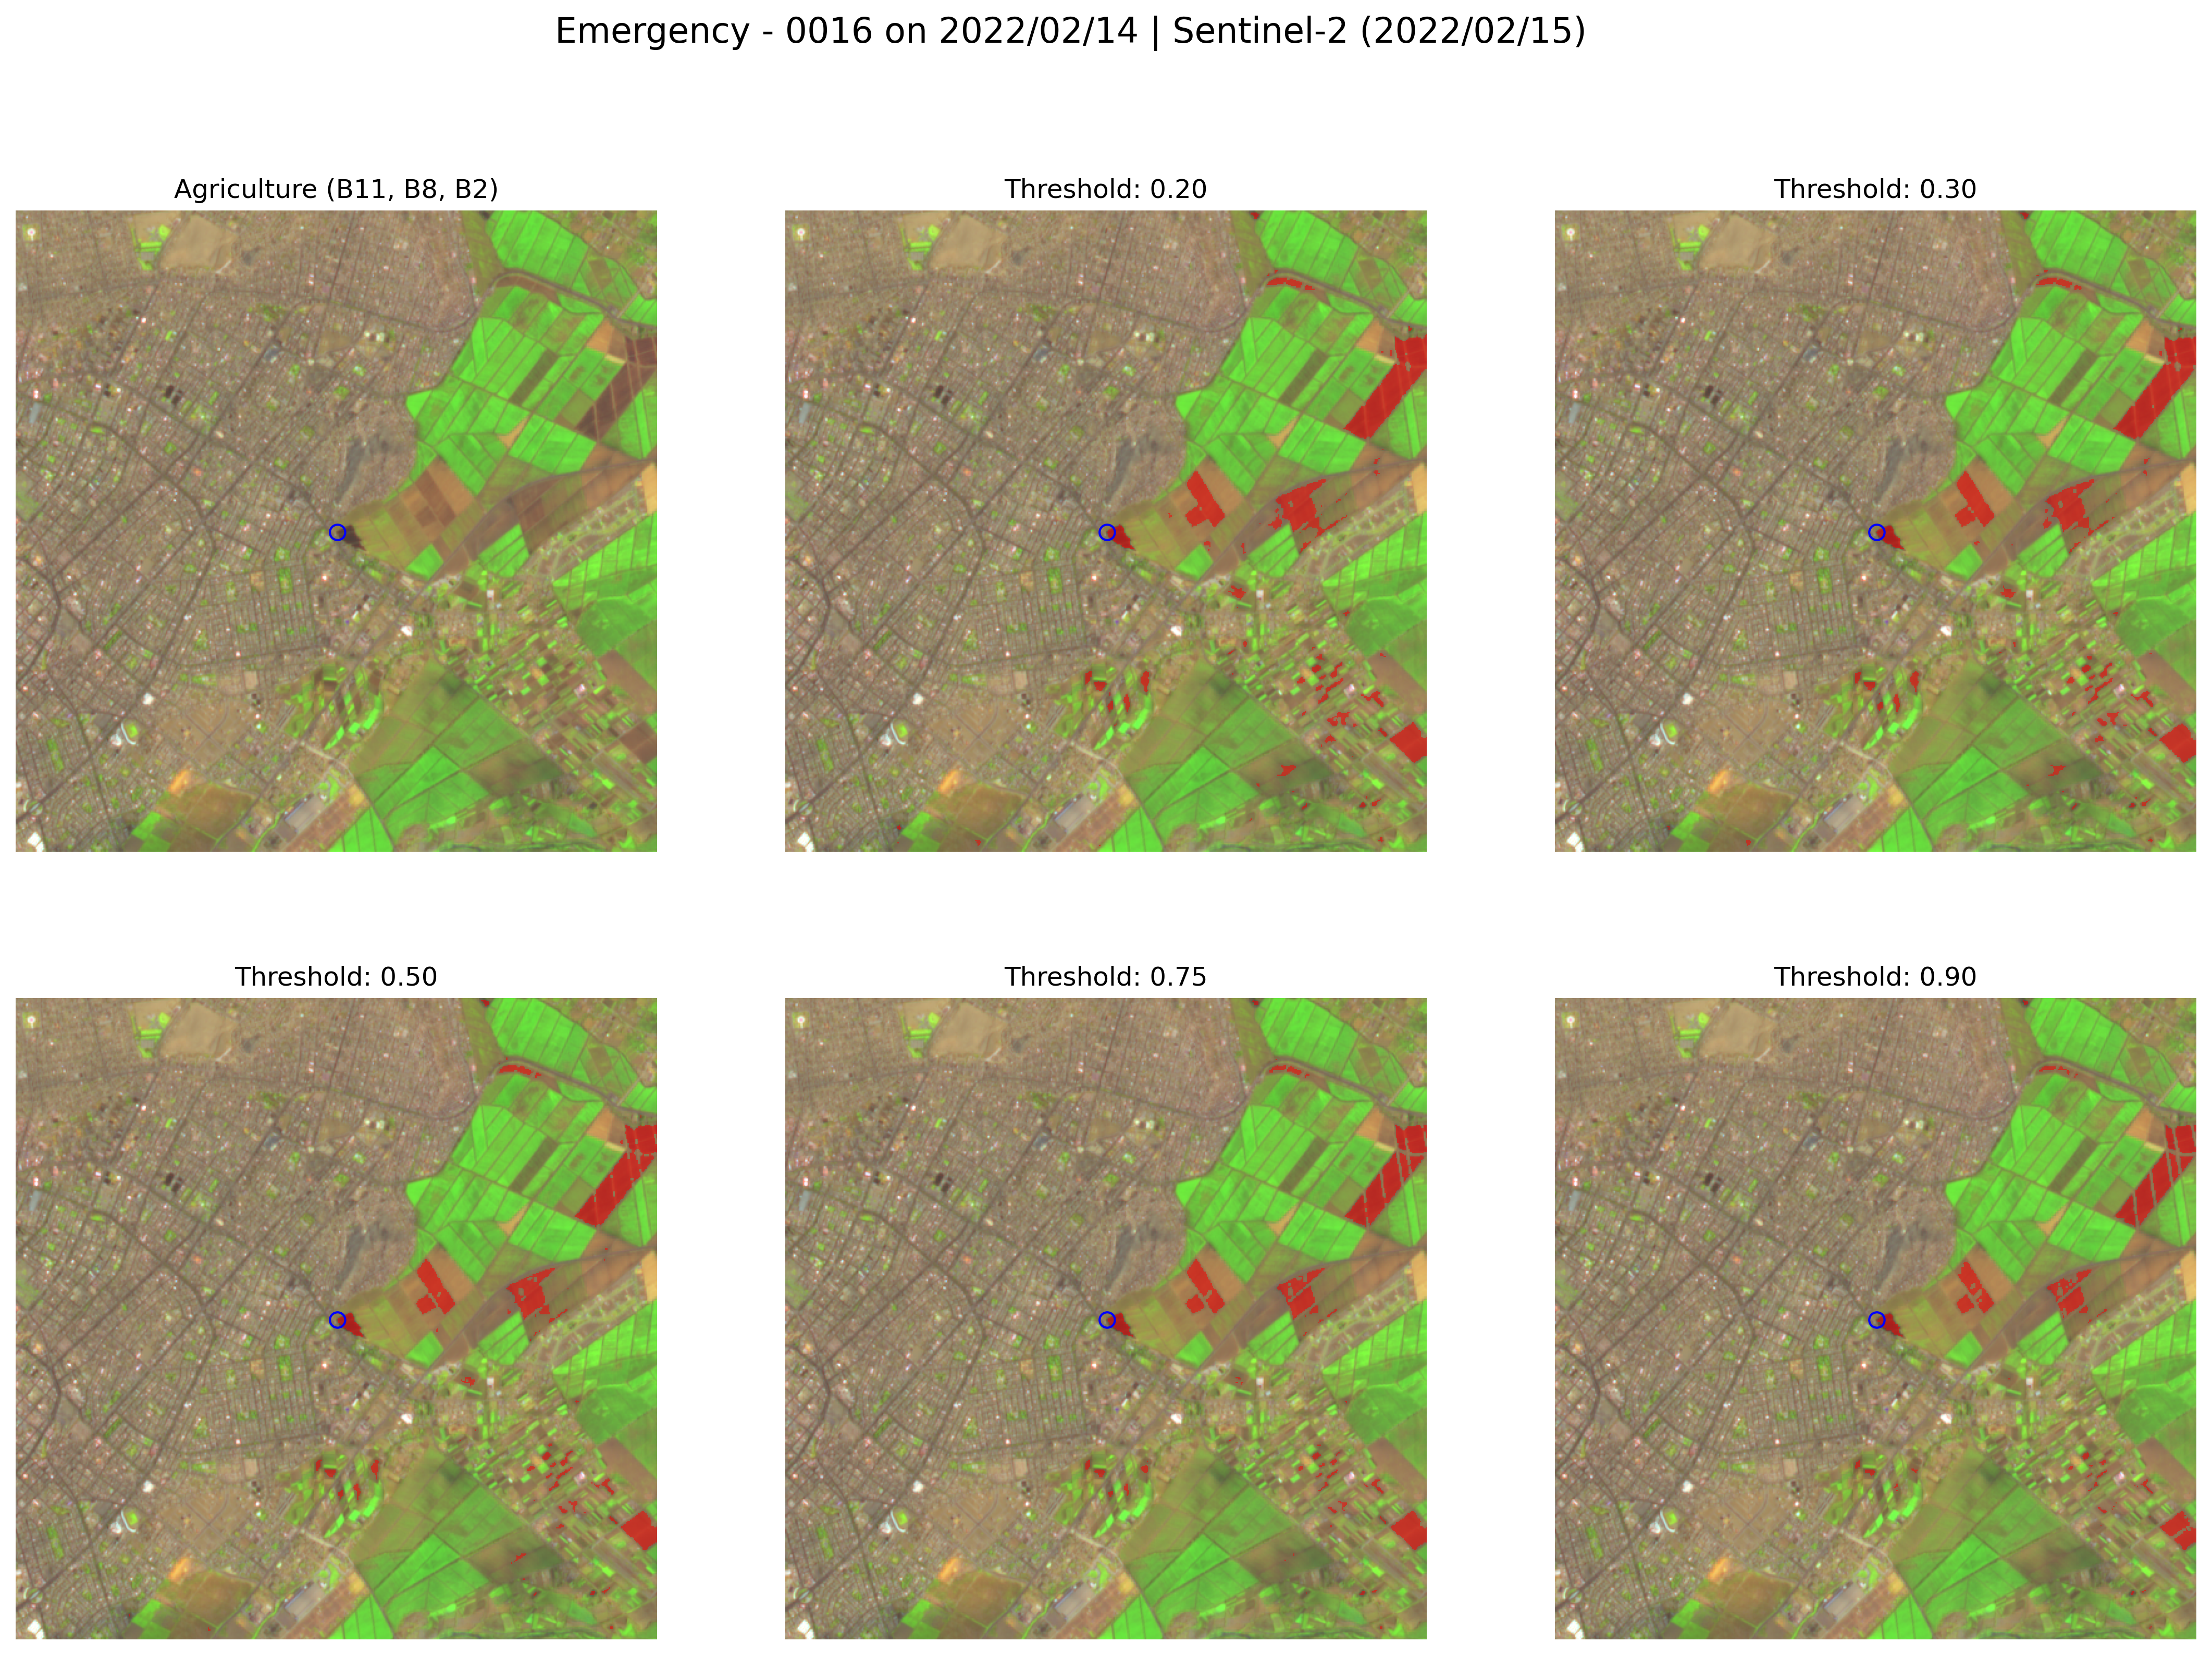
\includegraphics[width=0.9\textwidth]{img/7_resultados/0016.png}
    \begin{flushleft}
        \vspace{-\baselineskip}
        \textit{Nota.} Elaboración propia.
        \vspace{-\baselineskip}
    \end{flushleft}
\end{figure}

En la ciudad de Chicama, se reportó una emergencia \textbf{0376} en el campo San Jorge, propiedad de Agroindustrial Casa Grande S.A.A., debido a una quema accidental. 
En la imagen, se delimita un área de quema distribuida en nueve campos de cultivo. En este caso, como en la mayoría de los casos, 
los umbrales no se ven afectados, con el umbral en $0.20$ se estimó la ubicación y delimitación de la quema en un total de $13.94$ ha (Figura \ref{fig:comparacion_umbrales_0376}).

\begin{figure}[H]
    \centering
    \caption{Comparación de umbrales de probabilidad para la emergencia 0376.}
    \label{fig:comparacion_umbrales_0376}
    \includegraphics[width=0.9\textwidth]{img/7_resultados/0376.png}
    \begin{flushleft}
        \vspace{-\baselineskip}
        \textit{Nota.} Elaboración propia.
        \vspace{-\baselineskip}
    \end{flushleft}
\end{figure}

En la ciudad de Casa Grande, se reportó una emergencia \textbf{0068} en un área de 9 hectáreas 
perteneciente a Agroindustrial Casa Grande S.A.A., debido a una quema accidental. En este caso, 
la quema no fue intensa y se vió afectada por la presencia de vegetación que aún no había sido 
cosechada. Los umbrales más bajos ($0.20$ - $0.50$) lograron delimitar claramente el área afectada
con un total de $4.5$ ha, mientras que los umbrales más altos ($0.70$ y $0.90$) subestimaban estas
áreas (Figura \ref{fig:comparacion_umbrales_0068}). 

\begin{figure}[H]
    \centering
    \caption{Comparación de umbrales de probabilidad para la emergencia 0068.}
    \label{fig:comparacion_umbrales_0068}
    \includegraphics[width=0.9\textwidth]{img/7_resultados/0068.png}
    \begin{flushleft}
        \vspace{-\baselineskip}
        \textit{Nota.} Elaboración propia.
        \vspace{-\baselineskip}
    \end{flushleft}
\end{figure}

La emergencia \textbf{0456} en los campo de cultivo Bambas 2, perteneciente a Agroindustrial Laredo S.A.A., reportó una quema accidental que afectó 10 hectáreas de campo. En este caso, los umbrales más 
bajos ($0.20$ - $0.30$) tendieron a sobrestimar el área de quema debido a la reciente actividad y la presencia de suelo desnudo. Por lo tanto, un umbral alto de $0.90$ se considera el más adecuado 
para este escenario logrando delimitar un área de $10.29$ ha (Figura \ref{fig:comparacion_umbrales_0456}).

\begin{figure}[H]
    \centering
    \caption{Comparación de umbrales de probabilidad para la emergencia 0456.}
    \label{fig:comparacion_umbrales_0456}
    \includegraphics[width=0.9\textwidth]{img/7_resultados/0456.png}
    \begin{flushleft}
        \vspace{-\baselineskip}
        \textit{Nota.} Elaboración propia.
        \vspace{-\baselineskip}
    \end{flushleft}
\end{figure}

\subsection{Inferencia en el área piloto.}
El área analizada corresponde a los fundos azucareros cercanos a la ciudad de Laredo, durante un período reciente que abarca desde enero de 2023 hasta agosto de 2024. A partir de un total de 30 imágenes disponibles 
para esta área, se han generado tres series temporales.

\subsubsection{Marzo a junio de 2023.}
Durante los meses de marzo y junio de 2023 (Figura \ref{fig:inference_marzo_junio}), el análisis del 11 de mayo identificó $5.65$ ha de áreas quemadas pertencientes a dos campos de cultivo contiguos (recuadro celeste). Estas áreas, que cinco días antes eran suelos desnudos (zonas amarillentas), 
fueron requemadas debido a la presencia de paja o residuos de caña de azúcar. Para el 15 de junio, las áreas quemadas se vuelven más tenues, indicando que el suelo ha sido reacondicionado y preparado 
para la siembra.

\begin{figure}[H]
    \centering
    \caption{Resultados de la inferencia en el área piloto (Marzo a Junio de 2023).}
    \label{fig:inference_marzo_junio}
    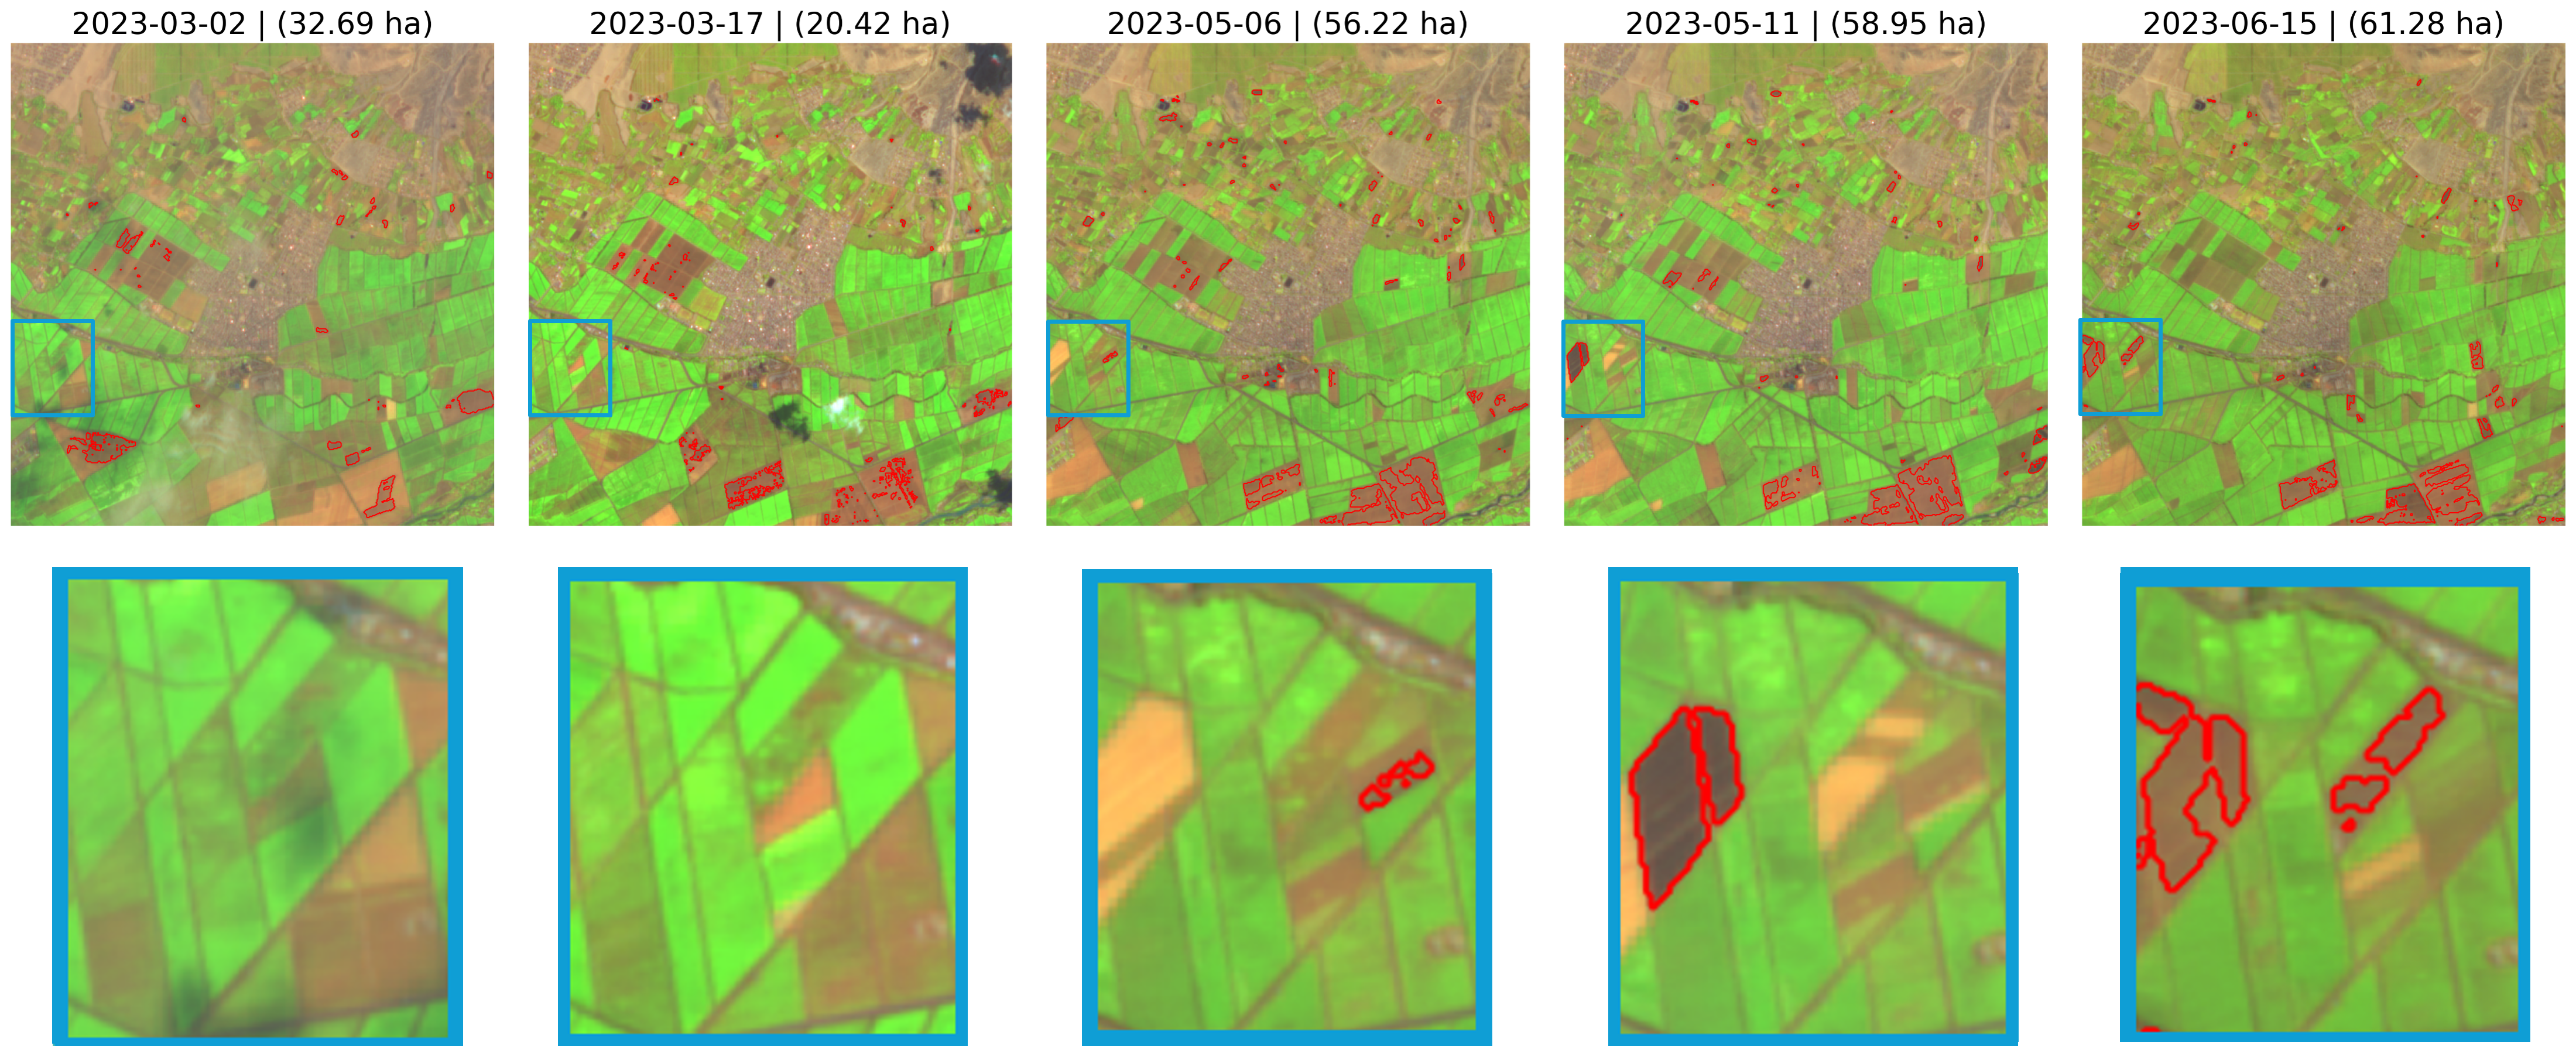
\includegraphics[width=1\textwidth]{img/7_resultados/timeseries_2023-05-06.png}
    \begin{flushleft}
        \textit{Nota.} Los valores de umbral utilizados fueron $0.85, 0.98, 0.75, 0.75, 0.75$ respectivamente. Elaboración propia.
        \vspace{-\baselineskip}
    \end{flushleft}
\end{figure}
    
\subsubsection{Octubre a noviembre de 2023.}
Durante los meses de octubre y noviembre de 2023 (Figura \ref{fig:inference_octubre_noviembre}), el análisis del 18 de octubre reveló $4.88$ ha de áreas quemadas recientemente en cuatro campo de cultivos cercanos (recuadro celeste), que hace cinco días eran suelo desnudo, similar
al caso anterior fue producto de la requema. En las tres fechas posteriores, estas áreas, aunque con menor intensidad, continúan siendo detectadas por el modelo.

Para el 22 de noviembre, se identificó un área con quema activa de $2.94$ ha, la cual cinco días después se observa con un tono más tenue y una extensión de $4.61$ ha.

\begin{figure}[H]
    \centering
    \caption{Resultados de la inferencia en el área piloto (Octubre a Noviembre de 2023).}
    \label{fig:inference_octubre_noviembre}
    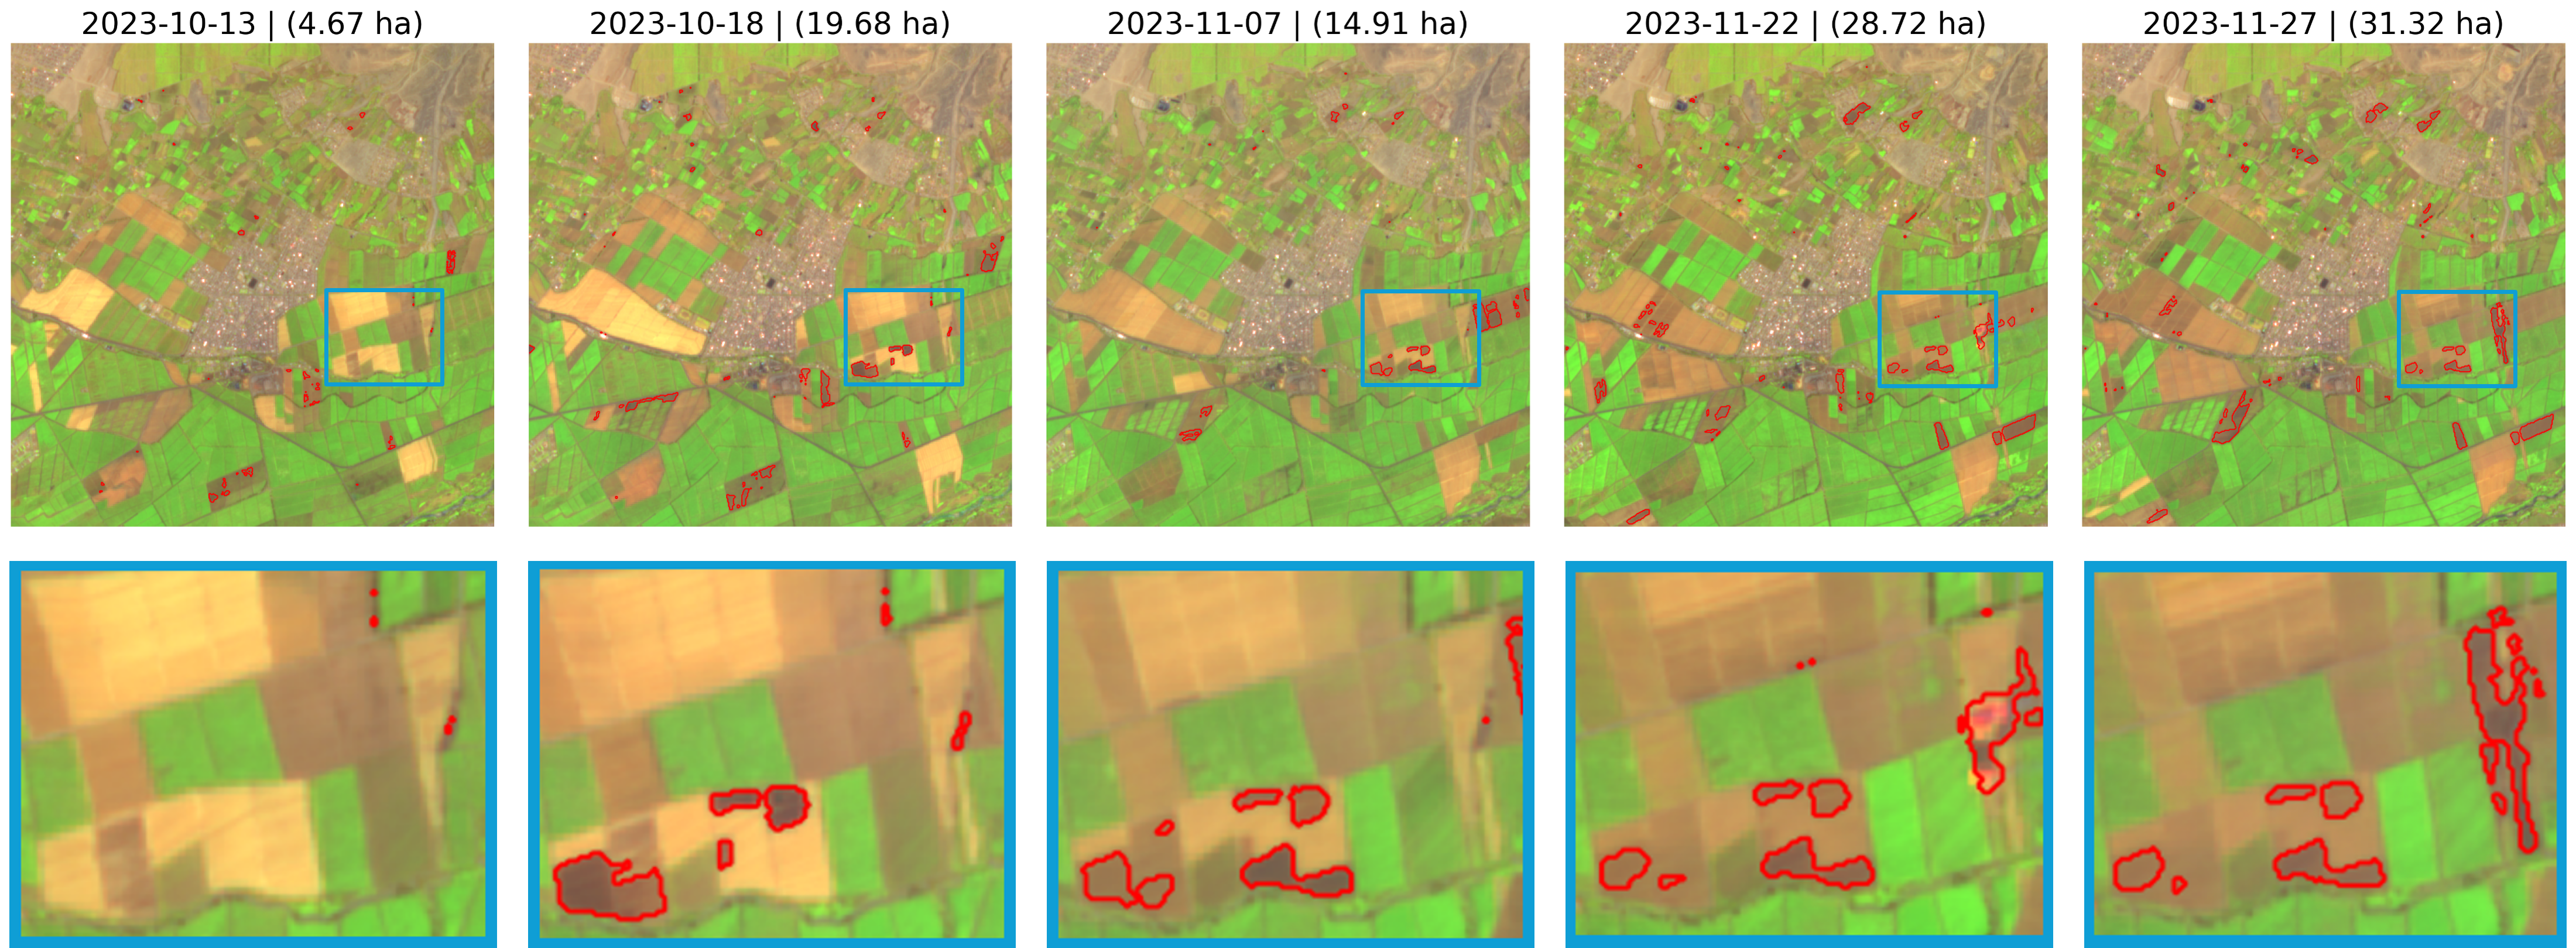
\includegraphics[width=1\textwidth]{img/7_resultados/timeseries_2023-11-07.png}
    \begin{flushleft}
        \textit{Nota.} Los valores de umbral utilizados fueron $0.85, 0.80, 0.80, 0.80, 0.80$ respectivamente. Elaboración propia.
        \vspace{-\baselineskip}
    \end{flushleft}
\end{figure}
    
\subsubsection{Marzo a abril de 2024.}
El análisis temporal durante los meses de marzo y abril de 2024 (Figura \ref{fig:inference_marzo_abril}),  muestra diferentes escenarios de quema: el recuadro amarillo identifica una pequeña quema activa de $0.64$ hectáreas el 15 de abril, que se atenúa 
cinco días después, pero sigue siendo detectada. 

El recuadro azul muestra tres áreas quemadas con un total de 9.75 hectáreas, que también se vuelven más tenues cinco días después. 

En el recuadro celeste se destaca áreas quemadas en dos campos contiguos el 26 de marzo, donde 
cinco días antes se observaba caña adulta, y un mes después de este evento, se encuentran recuperadas para la siembra y no son delimitadas por el modelo. Asímismo, otra área quemada se detecta el 15 de abril en un campo de cultivo donde se observa suelo desnudo
producto de la cosecha, que cinco días después se muestra más tenue y se está reacondicionando para la siembra.

\begin{figure}[H]
    \centering
    \caption{Resultados de la inferencia en el área piloto (Marzo a Abril de 2024).}
    \label{fig:inference_marzo_abril}
    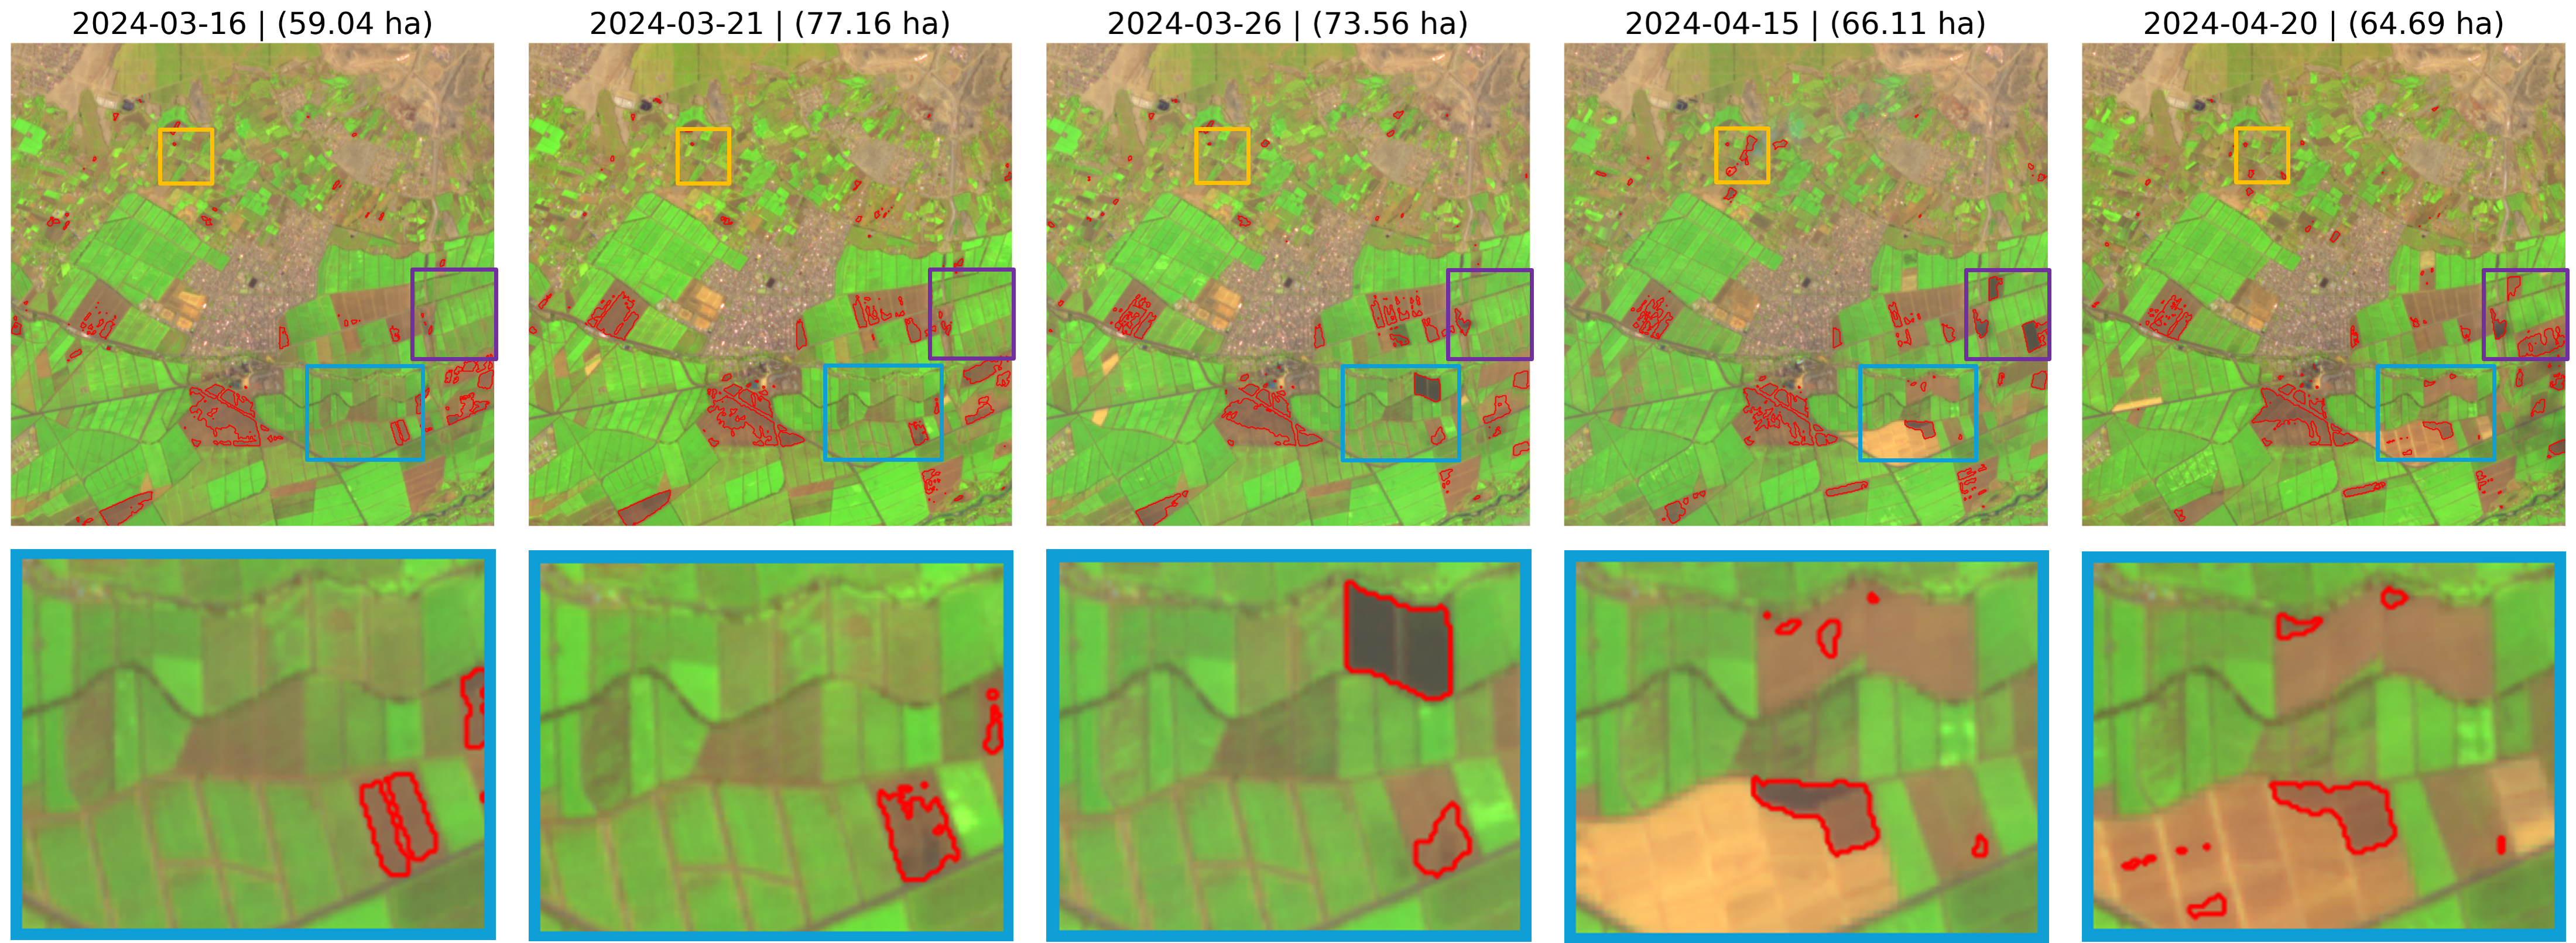
\includegraphics[width=1\textwidth]{img/7_resultados/timeseries_2024-03-26.png}
    \begin{flushleft}
        \textit{Nota.} Los valores de umbral utilizados fueron $0.85, 0.75, 0.75, 0.80, 0.80$ respectivamente. Elaboración propia.
        \vspace{-\baselineskip}
    \end{flushleft}
\end{figure}


